\section{Notions of linear separability}
\label{section:notions-of-linear-separability}

We define two notions of linear separability for multiclass classification. The
first notion is the standard notion of linear separability used in the proof of
the mistake bound for the \textsc{Multiclass Perceptron} algorithm. The second
notion is stronger, i.e. more restrictive. However, it is more suitable for the
bandit setting, since it allows for a simple and efficient algorithm; see
Section~\ref{section:algorithm-for-strongly-linearly-separable-data}.

\begin{definition}[Linear separability]
Let $(V,\ip{\cdot}{\cdot})$ be an inner product space, $K$ be a positive
integer, and $\gamma$ be a positive real number. Let $(x_1, y_1), (x_2,
y_2), \dots, (x_T, y_T)$ be labeled examples in $V \times \{1,2,\dots,K\}$.

The examples are said to be \emph{linearly separable with a
margin $\gamma$} if there exist vectors $w_1, w_2, \dots, w_K \in V$ such
that
\begin{align}
\label{equation:linear-separability-1}
\sum_{i=1}^K \norm{w_i}^2 & \le 1 \; , \\
\label{equation:linear-separability-2}
\forall t \in \{1,2,\dots,T\} \quad \forall i \in \{1,2,\dots, K\} \setminus \{y_t\} \qquad \qquad \ip{x_t}{w_{y_t}} & \ge \ip{x_t}{w_i} + \gamma \; .
\end{align}
\label{def:linear-sep}
\end{definition}

\begin{definition}[Strong Linear separability]
Let $(V,\ip{\cdot}{\cdot})$ be an inner product space, $K$ be a positive
integer, and $\gamma$ be a positive real number. Let $(x_1, y_1), (x_2,
y_2), \dots, (x_T, y_T)$ be labeled examples in $V \times \{1,2,\dots,K\}$.

The examples are said to be \emph{strongly linearly separable with a
margin $\gamma$} if there exist vectors $w_1, w_2, \dots, w_K \in V$ such
that
\begin{align}
\label{equation:strong-linear-separability-1}
\sum_{i=1}^K \norm{w_i}^2 & \le 1 \; , \\
\label{equation:strong-linear-separability-2}
\forall t \in \{1,2,\dots,T\} \qquad \qquad \ip{x_t}{w_{y_t}} &\ge \gamma \; , \\
\label{equation:strong-linear-separability-3}
\forall t \in \{1,2,\dots,T\} \qquad \forall i \in \{1,2,\dots, K\} \setminus \{y_t\} \qquad \qquad \ip{x_t}{w_i} & \le - \gamma \; .
\end{align}
\label{def:strong-linear-sep}
\end{definition}

The notion of linear separability with a margin is standard. It is used in the
full-information setting to upper bound the number of mistakes of the
\textsc{Multiclass Perceptron} algorithm. For completeness, we state the
algorithm in Appendix~\ref{section:multiclass-perceptron-proofs}. It is a
folklore result that if a set of labeled examples is separable with a margin
$\gamma$ and the norm of the examples is bounded by $R$ then \textsc{Multiclass
Perceptron} algorithm makes at most $\left\lfloor 2(R/\gamma)^2 \right \rfloor$
mistakes. Another folklore result is that \textsc{Multiclass Perceptron} is
essentially optimal in the sense that any deterministic algorithm must make
$\left\lfloor (R/\gamma)^2 \right \rfloor$ mistakes in the worst case. For
completeness, we give proofs of both of these results in
Appendix~\ref{section:multiclass-perceptron-proofs}.

The notion of strong linear separability is new.
\chicheng{I think the notion has appeared in~\cite{Chen-Chen-Zhang-Chen-Zhang-2009}, however,
they proposed an algorithm that doesn't achieve a finite mistake bound in the bandit
setting under this assumption (although they claimed that they have done so, the proof was
wrong..)}

It is easy to see that if labeled examples are strongly linearly
separable with margin $\gamma$ then they are linearly separable with margin
$2\gamma$. Indeed, if $w_1, w_2, \dots, w_K \in V$
satisfy \eqref{equation:strong-linear-separability-1},
\eqref{equation:strong-linear-separability-2},
\eqref{equation:strong-linear-separability-3} then they satisfy
\eqref{equation:linear-separability-1} and
\eqref{equation:linear-separability-2} with margin $\gamma' = 2\gamma$.


Similarly, if $K=2$ and labeled examples are linearly separable with a margin
$\gamma$ then they are strongly linearly separable with margin $\gamma/2$.
Indeed, if $w_1, w_2$ satisfy \eqref{equation:linear-separability-1} and
\eqref{equation:linear-separability-2} then $w_1' = \frac{w_1 - w_2}{2}$, $w_2' =
\frac{w_2 - w_1}{2}$ and $\gamma'=\gamma/2$ satisfy
\eqref{equation:strong-linear-separability-1},
\eqref{equation:strong-linear-separability-2},
\eqref{equation:strong-linear-separability-3}. The last two conditions are easy
to see. The first condition follows from $\norm{w_i'}^2 \le (\frac{1}{2}
\norm{w_1} + \frac{1}{2} \norm{w_2})^2 \le \frac{1}{2}\norm{w_1}^2 +
\frac{1}{2}\norm{w_2}^2 \le \frac{1}{2}$ for $i=1,2$.

\chicheng{Shall we change the $\gamma$ in Equations \eqref{equation:strong-linear-separability-2}, \eqref{equation:strong-linear-separability-3} to $\gamma/2$, to simplify the presentation?}

However, for any $K \ge 3$ and any inner product space of dimension at least
$2$, there exists a set of labeled examples that is linearly separable with a
positive margin $\gamma$ but it is not strongly linearly separable with any
positive margin $\gamma$. An example of such set of labeled examples is shown in
Figure~\ref{figure:linearly-separable-examples-with-margin}.

\begin{figure}
\begin{center}
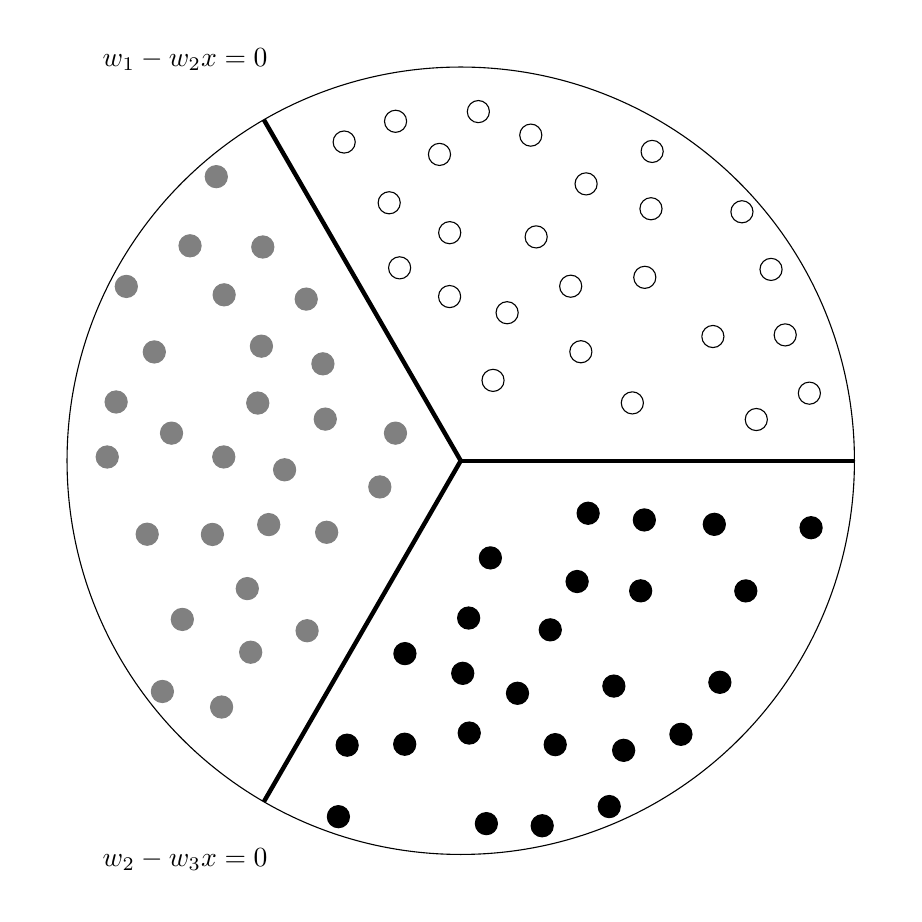
\begin{tikzpicture}

  \useasboundingbox (-5.5,-5.5) rectangle (5.5,5.5);
  % \draw[help lines] (-5.5,-5.5) rectangle (5.5,5.5);

  % Grid and coordinate axes
  %% \draw[help lines] (-5.2,-5.2) grid (5.2,5.2);
  %% \draw[thick, ->, >=latex] (-5.2,0) -- (5.2,0);
  %% \draw[thick, ->,  >=latex] (0,-5.2) -- (0,5.2);

  % Notable points
  \coordinate (Origin) at (0,0);

  \coordinate [label={[xshift=-10mm, yshift=5mm]$\ip{w_1 - w_2}{x} = 0$}] (A) at (120:5);
  \coordinate [label={[xshift=-10mm, yshift=-10mm]$\ip{w_2 - w_3}{x} = 0$}] (B) at (240:5);
  \coordinate [label={[xshift=+20mm, yshift=-3mm]$\ip{w_3 - w_1}{x} = 0$}] (C) at (360:5);

  % Circle which contains all the examples.
  \draw (Origin) circle (5);

  \draw[ultra thick] (Origin) -- (A);
  \draw[ultra thick] (Origin) -- (B);
  \draw[ultra thick] (Origin) -- (C);

  % Class 0 points. Angles between 0.0 and 120.0
  \draw[color=black, fill=none]
                    (7.94:3.79) circle (4pt)
                    (10.97:4.51) circle (4pt)
                    (18.63:2.30) circle (4pt)
                    (21.20:4.42) circle (4pt)
                    (26.23:3.57) circle (4pt)
                    (31.66:4.63) circle (4pt)
                    (41.52:4.77) circle (4pt)
                    (42.22:2.06) circle (4pt)
                    (44.90:3.30) circle (4pt)
                    (52.95:4.01) circle (4pt)
                    (57.79:2.62) circle (4pt)
                    (58.25:4.62) circle (4pt)
                    (65.64:3.86) circle (4pt)
                    (68.11:1.10) circle (4pt)
                    (71.38:3.00) circle (4pt)
                    (72.60:1.97) circle (4pt)
                    (77.86:4.23) circle (4pt)
                    (87.11:4.44) circle (4pt)
                    (92.77:2.90) circle (4pt)
                    (93.88:2.09) circle (4pt)
                    (93.97:3.90) circle (4pt)
                    (100.87:4.39) circle (4pt)
                    (105.50:3.40) circle (4pt)
                    (107.58:2.57) circle (4pt)
                    (110.09:4.31) circle (4pt)
                    ;

  % Class 1 points. Angles between 120.0 and 240.0
  \draw[color=gray, fill=gray]
                    (130.71:4.76) circle (4pt)
                    (132.80:3.70) circle (4pt)
                    (133.71:2.84) circle (4pt)
                    (141.55:4.39) circle (4pt)
                    (144.89:2.14) circle (4pt)
                    (144.96:3.67) circle (4pt)
                    (150.11:2.92) circle (4pt)
                    (152.47:4.79) circle (4pt)
                    (157.09:0.90) circle (4pt)
                    (160.45:4.13) circle (4pt)
                    (162.92:1.80) circle (4pt)
                    (164.13:2.68) circle (4pt)
                    (170.32:4.44) circle (4pt)
                    (174.55:3.69) circle (4pt)
                    (179.08:3.01) circle (4pt)
                    (179.39:4.49) circle (4pt)
                    (182.94:2.24) circle (4pt)
                    (193.19:4.09) circle (4pt)
                    (196.53:3.29) circle (4pt)
                    (197.93:1.08) circle (4pt)
                    (198.39:2.57) circle (4pt)
                    (208.08:1.93) circle (4pt)
                    (209.68:4.07) circle (4pt)
                    (210.92:3.16) circle (4pt)
                    (217.72:4.79) circle (4pt)
                    (222.35:3.61) circle (4pt)
                    (225.84:4.36) circle (4pt)
                    (227.89:2.91) circle (4pt)
                    ;

% Class 2 points. Angles between 240.0 and 360.0
  \draw[color=black, fill=black]
                    (248.23:3.89) circle (4pt)
                    (251.03:4.78) circle (4pt)
                    (253.86:2.55) circle (4pt)
                    (258.82:3.67) circle (4pt)
                    (270.54:2.70) circle (4pt)
                    (271.79:3.46) circle (4pt)
                    (272.88:2.00) circle (4pt)
                    (274.04:4.62) circle (4pt)
                    (282.58:4.75) circle (4pt)
                    (283.72:3.04) circle (4pt)
                    (286.97:1.29) circle (4pt)
                    (288.41:3.80) circle (4pt)
                    (293.24:4.78) circle (4pt)
                    (297.90:2.43) circle (4pt)
                    (299.36:4.22) circle (4pt)
                    (304.20:3.46) circle (4pt)
                    (308.83:4.46) circle (4pt)
                    (313.94:2.13) circle (4pt)
                    (319.47:4.33) circle (4pt)
                    (324.13:2.82) circle (4pt)
                    (335.46:3.98) circle (4pt)
                    (337.60:1.75) circle (4pt)
                    (342.13:2.45) circle (4pt)
                    (345.92:3.32) circle (4pt)
                    (349.18:4.53) circle (4pt)
                    ;

\end{tikzpicture}

\end{center}
\caption[]{The figure shows labeled examples in $\R^2$. The examples belong to
$K=3$ classes colored white, gray and black respectively. Each class lies in a
$120^\circ$ wedge. In other words, each class lies in an intersection of two
halfspaces.

While the examples are linearly separable with a positive margin $\gamma$, they
are \emph{not} strongly linearly separable with any positive margin $\gamma$.
}
\label{figure:linearly-separable-examples-with-margin}
\end{figure}
